\chapter{Mobile Ad Hoc Network Visualization}
\label{chap:network_vis}

\section{Introduction}
The process of visualizing mobile ad hoc networks is a particularly important and challenging task. This is due to the fact that these types of networks are highly dynamic and maintain no fixed structure.  The simulation of these networks is a complex process that has many different layers to understand and monitor.  Visualizing information about the different layers and parameters used in simulation can help improve the understanding of these networks and the simulated results.

In this chapter we present two different visualizations.  First we present a method of visualizing signal radiation patterns at the physical layer of the network model.  These radiation patterns originate from transmitting nodes and are used to indicate how strong their signal is in the areas surrounding them.  This pattern can be affected by a number of things such as interference from other transmitting nodes in the vicinity.  Properly visualizing these radiation patterns can help us understand the effects of various parameter selections on network performance.

We then present the use of digital terrain to enhance the visualization and simulation of ad hoc mobile networks.  A discussion of a library for handling digital terrain data is given, as well as how this library is integrated into the mobile ad hoc network simulator OMAN.  The visualization options this new library offers are also discussed.

\section{Related Work}
The technical literature on the visualization of ad hoc networks is significantly limited. To the best of our knowledge, existing work is restricted to small-scale examples that focus more on the attainment of the data that is visualized and less on the clarity, quality, and richness of information contained in the visual output \cite{DhoVoGue03}. Connectivity is a critical metric for performance of ad hoc networks, and is easy to visualize, even as the size of the network scales up. Therefore, most larger scale visual information processing efforts in the networking and visualization literature are focused on connectivity, such as in \cite{Bettsetetter04, HamWij04, BecEicWil95, HerMelMar00}. On the other hand, tools that allow for the visualization of other aspects of the communication medium can only handle small scale networks, both in terms of running-time complexity and visual complexity; \cite{FitSeeRei04, MatBieLau05, EstHanHei00} are popular examples of such tools.

The use of digital terrain data in ad hoc network simulation is becoming more popular as it increases the realism of the simulations.  The work done by \cite{LuiPerNic01}, \cite{BonWanSta98}, and \cite{DzaTraFil07} all have modules that accounts for the use of digital terrain data in computing the propagation of the radio waves in their simulations.  They use digital terrain to extract terrain profiles for a given path between two nodes.  These profiles are then used in computing their propagation models.  Unfortunately, none of these works make use of this terrain data for effectively visualizing the results of their simulations.  The focus and novelty of the visualization methods presented here are in the effective visual representation of network resources and simulation results.


\section{Signal Radiation Pattern Visualization}
\subsection{Network Model}
The main goal of this task was to provide a visualization for the physical (PHY) layer of the networking model as defined by \cite{WuChoQia05}.  The PHY layer has two parameters associated with it.  First, is the fixed transmission power $P_i$ on each node $i$.  Second, is the minimum acceptable signal-to-interference-plus-noise (SINR) ratio, $\gamma$.  The SINR value from transmitter $i$ to receiver $j$ in time slot $z$ is given by
\begin{equation}
SINR_{ij}(z) = \frac{P_i A_{ij}}{\sum_{k \in V_P^z / i} P_k A_{k j} + \eta } , (i, j) \in E_P^z , z = 1,...,m
\end{equation} 

where $\eta$ is the channel noise power.  The channel attenuation between transmitter $i$ and receiver $j$ is 

\begin{equation}
A_{ij} = (\frac{d_{ref}}{d_{ij}})^\alpha
\end{equation}

where $d_{ij}$ is the distance between nodes $i$ and $j$, $d_{ref}$ is a channel reference distance, and $\alpha$ is the attenuation exponent.  All edges $(i,j)$ in each graph $G_P^z$ satisfy the requirement that \begin{math}SINR_{ij}(z) > \eta \end{math}.

\subsection{Visualization}
This model defines the parameters that are then visualized to show the signal radiation patterns from transmitting nodes.  This visualization takes into account two different models of the channel.  The first is a channel state that is assumed to be fully known with no fading, shadowing, or noise in the computation of the attenuation.  The second model is that of a highly unstable state, modeling uncertainty in the attenuation exponent, shadowing, fading, node positions, and noise.

\begin{figure} [ht]
%\begin{center}
\centering
	\subfigure[]{
		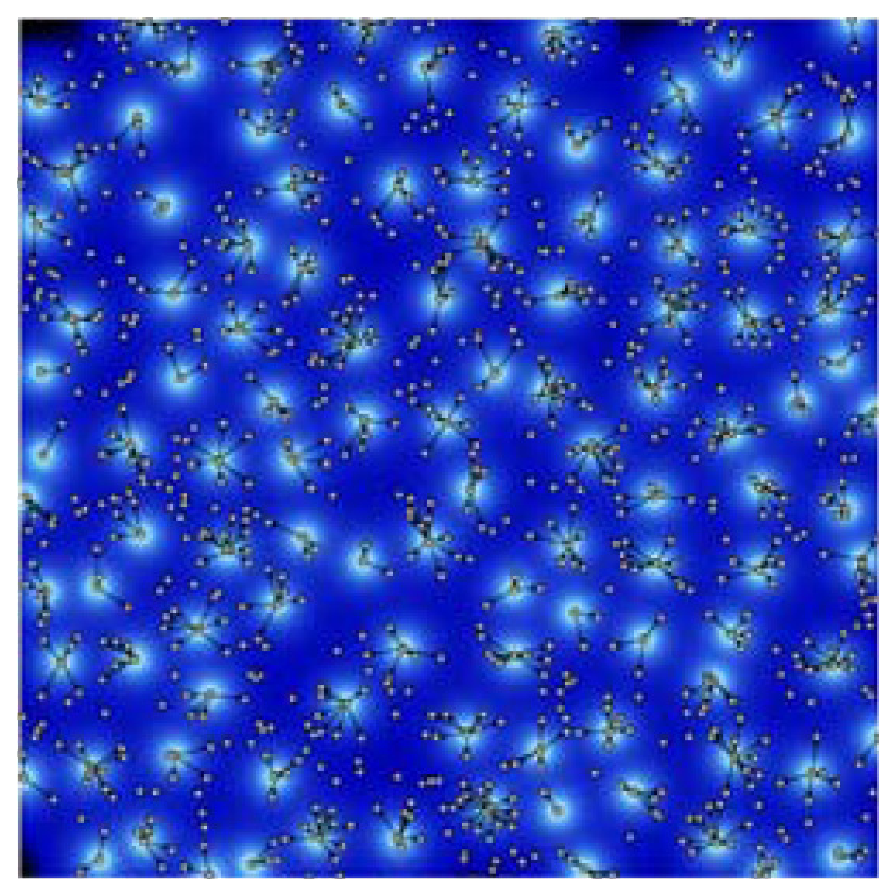
\includegraphics[scale=0.45]{images/network_vis/rad_pat_certain.eps}
		\label{fig:rad_pat_certain}
	}
	\subfigure[]{
		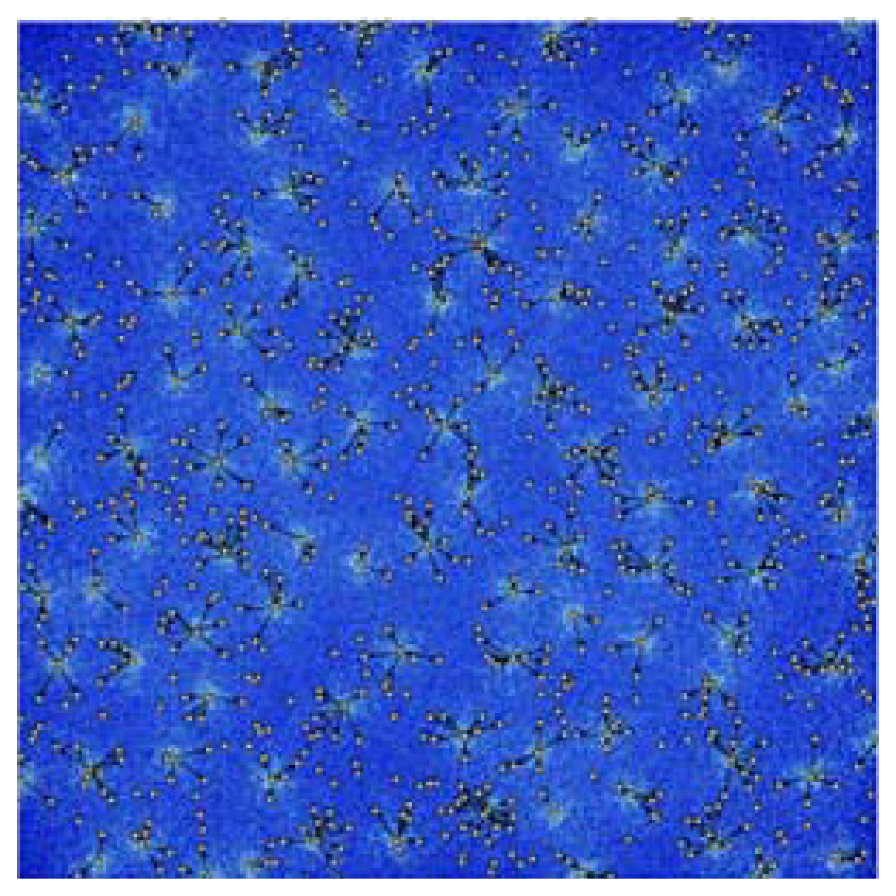
\includegraphics[scale=0.45]{images/network_vis/rad_pat_uncertain.eps}
		\label{fig:rad_pat_uncertain}
	}
%\end{center}
\caption{Signal radiation patterns for the two channel state models, \subref{fig:rad_pat_certain} fully known channel state, \subref{fig:rad_pat_uncertain} highly unstable channel state.}
\label{fig:rad_pat}
\end{figure}

The signal radiation patterns are shown by the change in color gradient as the signal gets weaker.  The gradient starts with white as the highest value and shifts into blue for intermediate values and finally to black for a zero valued signal.  Figure \ref{fig:rad_pat_certain} illustrates the fully known channel state model while Figure \ref{fig:rad_pat_uncertain} illustrates the highly unstable channel state model.  These two visual presentations of the physical state help demonstrate that it is much more difficult to make resource allocation decisions under uncertainty.

\begin{figure}[ht]
\begin{center}
	\subfigure[]{
		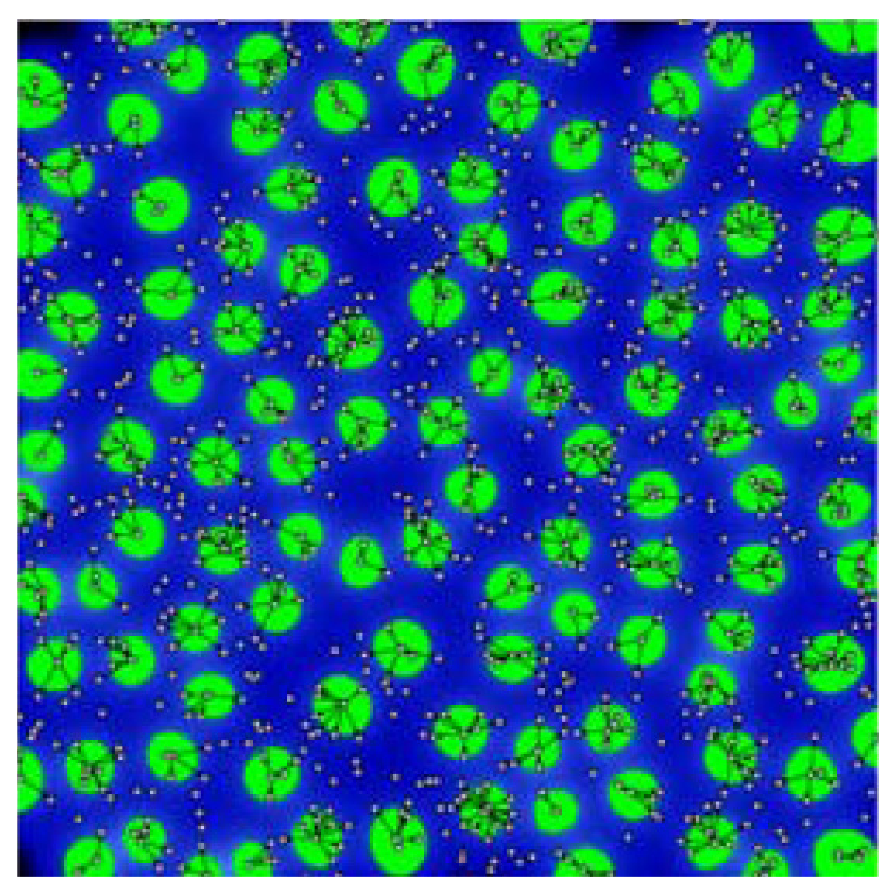
\includegraphics[scale=0.45]{images/network_vis/rad_pat_sinr_certain.eps}
		\label{fig:rad_pat_sinr_certain}
	}
	\subfigure[]{
		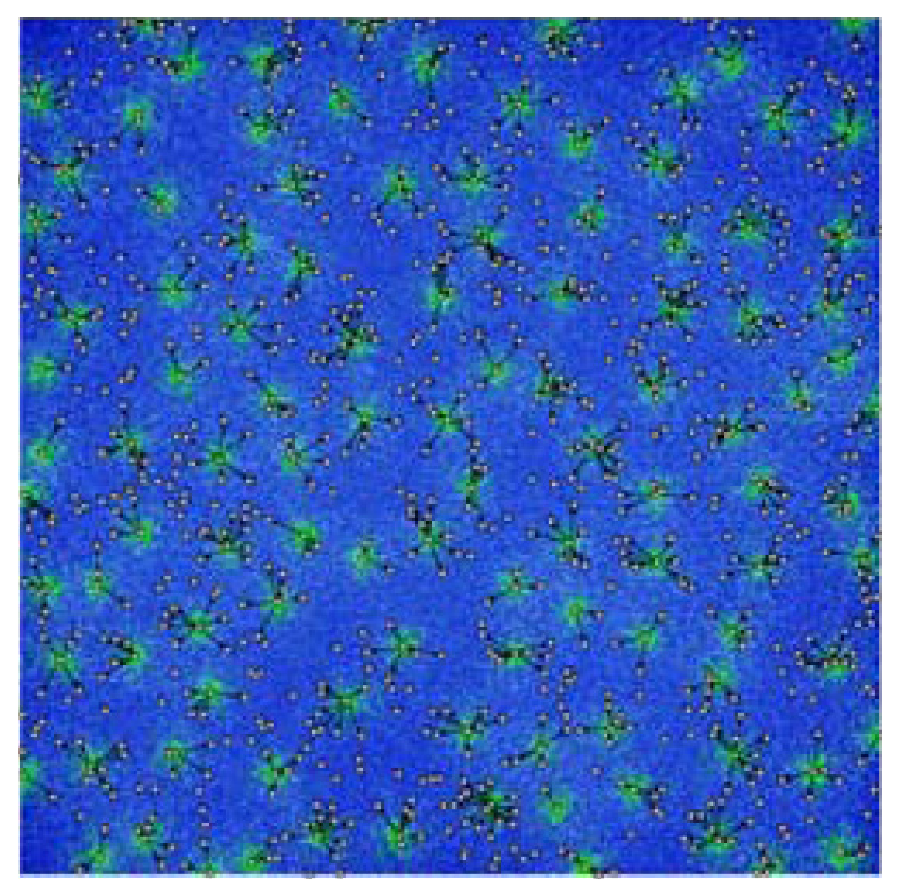
\includegraphics[scale=0.45]{images/network_vis/rad_pat_sinr_uncertain.eps}
		\label{fig:rad_pat_sinr_uncertain}
}
\end{center}
\caption{Acceptable SINR regions with signal radiation patterns for the two channel state models, \subref{fig:rad_pat_sinr_certain} fully known channel state, \subref{fig:rad_pat_sinr_uncertain} highly unstable channel state.}
\label{fig:rad_pat_sinr}
\end{figure}

We can also visualize the regions where the SINR is acceptably high for a feasible channel to exist.  That is, if a transmitter where to move into one of those regions, it would be able to transmit a signal to the receiving node associated with that region.  These areas are represented by bright green regions in the visualization.  These regions can have their translucency adjusted so the underlying signal radiation patterns can still be seen as desired.  Figure \ref{fig:rad_pat_sinr_certain} shows us these SINR regions in the fully known channel state model and Figure \ref{fig:rad_pat_sinr_uncertain} shows us these same regions in the highly unstable channel state model. Again we can see that the presence of uncertainty makes it difficult to design node movement and scheduling such that the receiver nodes can remain in the feasible regions of the transmitter with whom they seek to communicate.


\section{Digital Terrain Visualization}
The inclusion of digital terrain data in ad hoc network simulation is not new.  Terrain data is very commonly used while computing radio wave propagation models when simulating wireless networks.  For this reason the effort was made to integrate the use of digital terrain data into the OMAN ad hoc wireless network simulator.  The use of this data was primarily for use in more detailed calculations for running simulations, but also provides a more detailed visualization for the final results.  The following sections describe the efforts taken to create a system to manage terrain data transparently and the results of integrating that system with OMAN.

\subsection{Digital Terrain Library}
To facilitate the use of digital terrain data in the OMAN ad hoc network simulator, a library was developed to encapsulate the tasks required for managing and interacting with digital terrain data.  This library was designed to abstract away the details of the digital terrains file format and provide a standardized interface through which the desired data can be accessed.  Figure \ref{fig:terrain_lib_diagram} gives a general overview of the design structure of the terrain library.  The following sections will provide further details about each class.

\begin{figure}[ht]
\begin{center}
		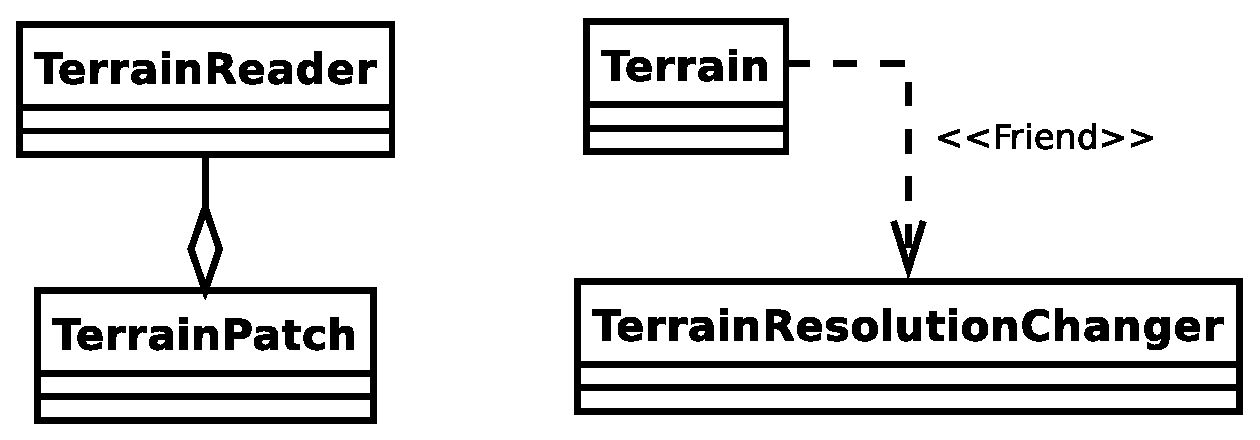
\includegraphics[scale=0.45]{images/network_vis/terrain_lib_diagram.eps}
\end{center}
\caption{UML diagram of the design of the terrain library.}
\label{fig:terrain_lib_diagram}
\end{figure}

\subsubsection{Terrain Class}
The Terrain class is the primary interface through which users interact with the terrain data.  The class presents the data like a large matrix where each cell contains an elevation value, measured in meters from sea level.  The origin of this matrix is defined to be the lower left corner.  The boundaries of this matrix are defined in two ways.  First the bounding box can be accessed as a set of latitude and longitude coordinates specifying the lower left and upper right corners of the bounding box.  The second method is to simply return the width and height of the area covered in meters.  Accessing the grid in this manner hides the details about the resolution of the terrain data since different file formats are of differing resolutions.

\paragraph{Accessing Terrain Elevations}
Knowing these standards for referencing coordinates within the terrain classes grid, users can access the actual elevation data is several different ways.  The first method allows them to sample a single point of elevation at any coordinate within the defined grid.  If the position they chose to sample does not contain a discrete elevation value, one will be interpolated using bilinear interpolation.

The second method of access allows the users to extract a sub-matrix of elevation data.  The user specifies the lower left and upper right coordinates of the bounding box of the desired sub-matrix.  If the coordinates of the users bounding box does not fall onto discrete values in the elevation matrix, the bounding box will be enlarged to the nearest set of discrete points that encompass the users original coordinates.  Figure \ref{fig:terrain_bb} provides an illustration of this mechanism.  Using this method of access, no interpolation will be done, only discrete elevation values will be returned.

\begin{figure}[ht]
\centering
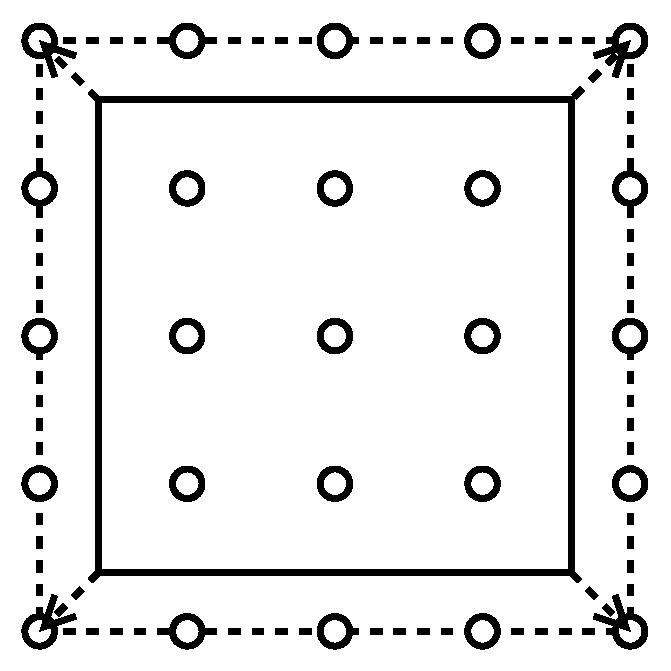
\includegraphics{images/network_vis/terrain_bounding_box.eps}
  \caption{The circle represent discrete points in the terrain grid.  The solid box is the users original desired bounding box.  The box is enlarged to the nearest discrete points that still encompass the original set of desired data.}
\label{fig:terrain_bb}
\end{figure}

The third method of access allows the users to generate terrain profiles along either a horizontal or vertical line.  The vertical profile takes two coordinates that define a straight line through the terrain and the number of points the user wants returned along this line.  A vector of elevation values is then returned with the desired number of points.  Elevation data points are interpolated as needed to fill out the desired sized vector.  A horizontal profile is generated by defining a region of interest with a bounding box and giving a cutoff elevation value.  This region of interest is then processed such that all points with elevation greater than or equal to the cutoff elevation remain and all others are dropped.  Once is done, polygons are created from the sets of remaining elevation points.  This set of polygons is then returned to the user.  Figure \ref{fig:terrain_horizontal_cut} illustrates this method.  Here all the white points are those that are above the cutoff elevation and the green lines draw out the polygons then defined by those regions.

\begin{figure}[ht]
\centering
  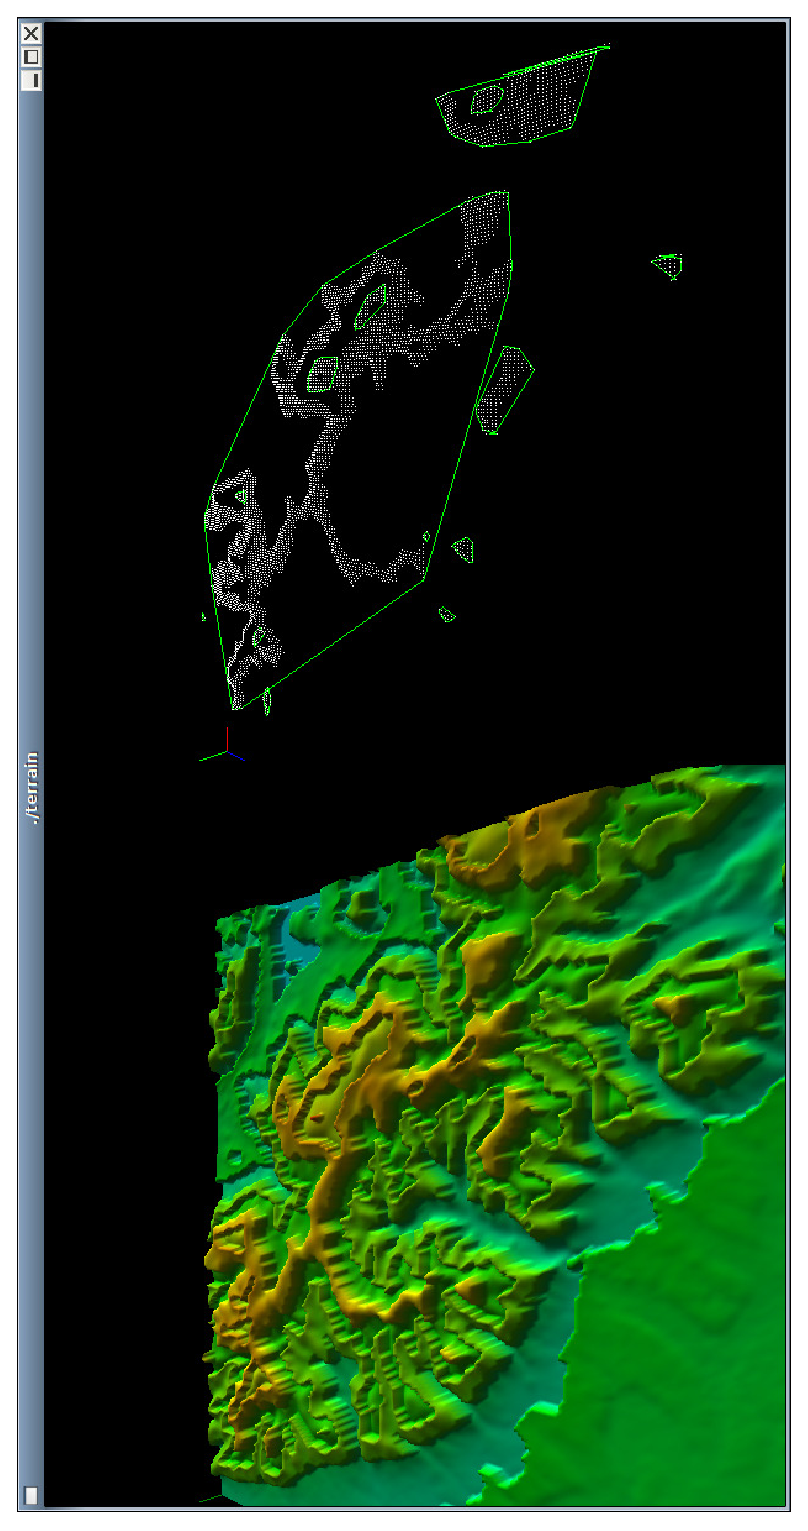
\includegraphics[angle=270,width=\linewidth]{images/network_vis/terrain_horizontal_cut.eps}
  \caption{Example of the results produced by a horizontal profile of a region of terrain.  The left side is the original terrain visualized in 3D.  The right side are the results of applying the horizontal profile method.}
\label{fig:terrain_horizontal_cut}
\end{figure}

\paragraph{Handling Water}
Most digital terrain file formats account for areas of water in some fashion.  This terrain library maintains a map of where any water resides within any loaded terrain data.  They user can then query the terrain class using an \textit{isWater()} function for any point within the grid and get a boolean response.

In most digital terrain file formats, the elevation values are measured from sea level.  Any zero valued terrain cells are then considered to be water.  Identifying these bodies of water is a simple search while loading the terrain data from the files.  Some digital terrain file formats, such as DTED, specify a means of identifying bodies of water that are not at sea level, such as lakes or reservoirs.  These bodies of water must be larger than a certain size in order to be captured in the terrain data.  This terrain library implements the proper algorithms for identifying these bodies of water and allowing the user access to them both for computation and visualization.

\begin{figure}[ht]
\centering

\subfigure[]{
	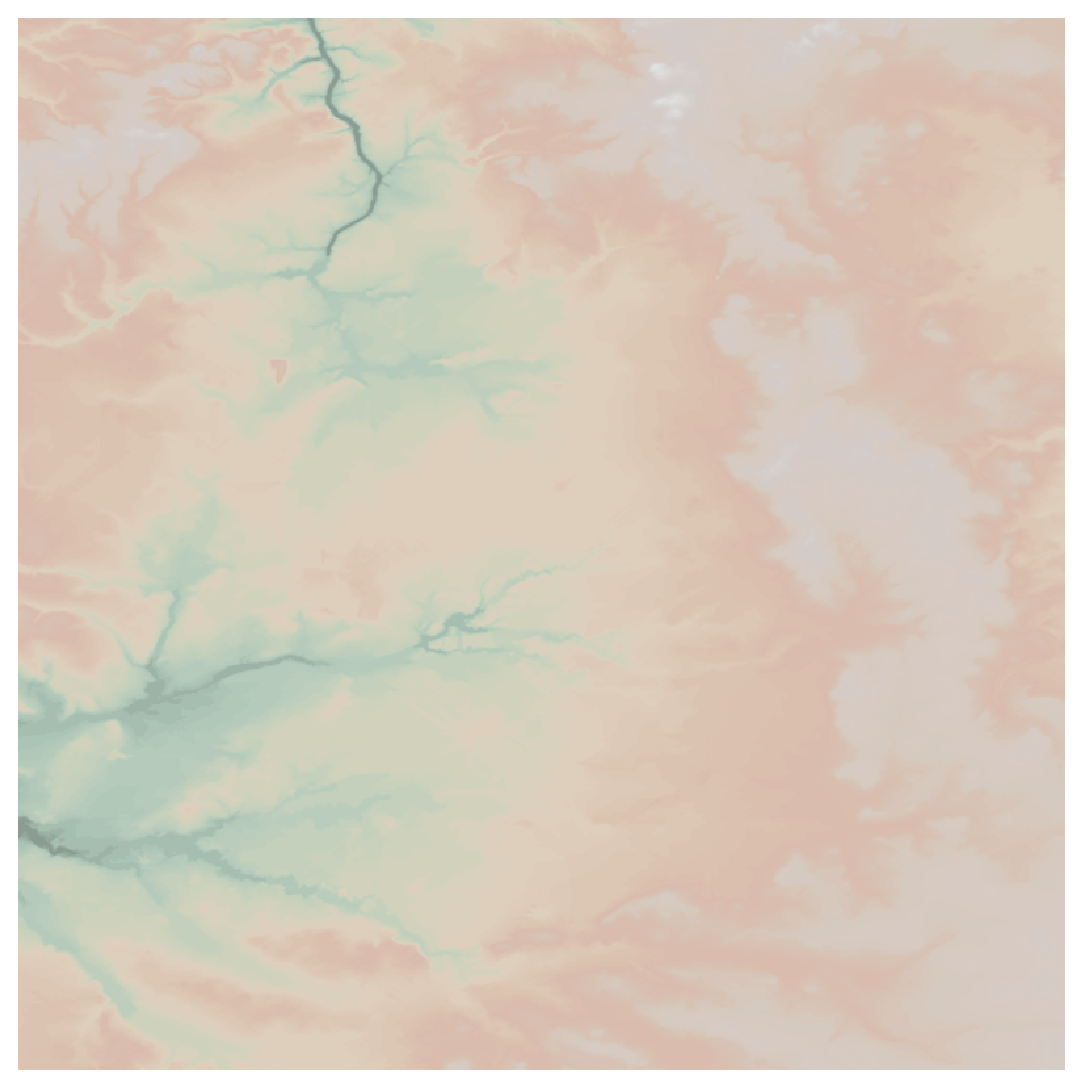
\includegraphics[scale=0.4]{images/network_vis/terrain_no_lakes.eps}
	\label{fig:terrain_no_lakes}
}
\subfigure[]{
	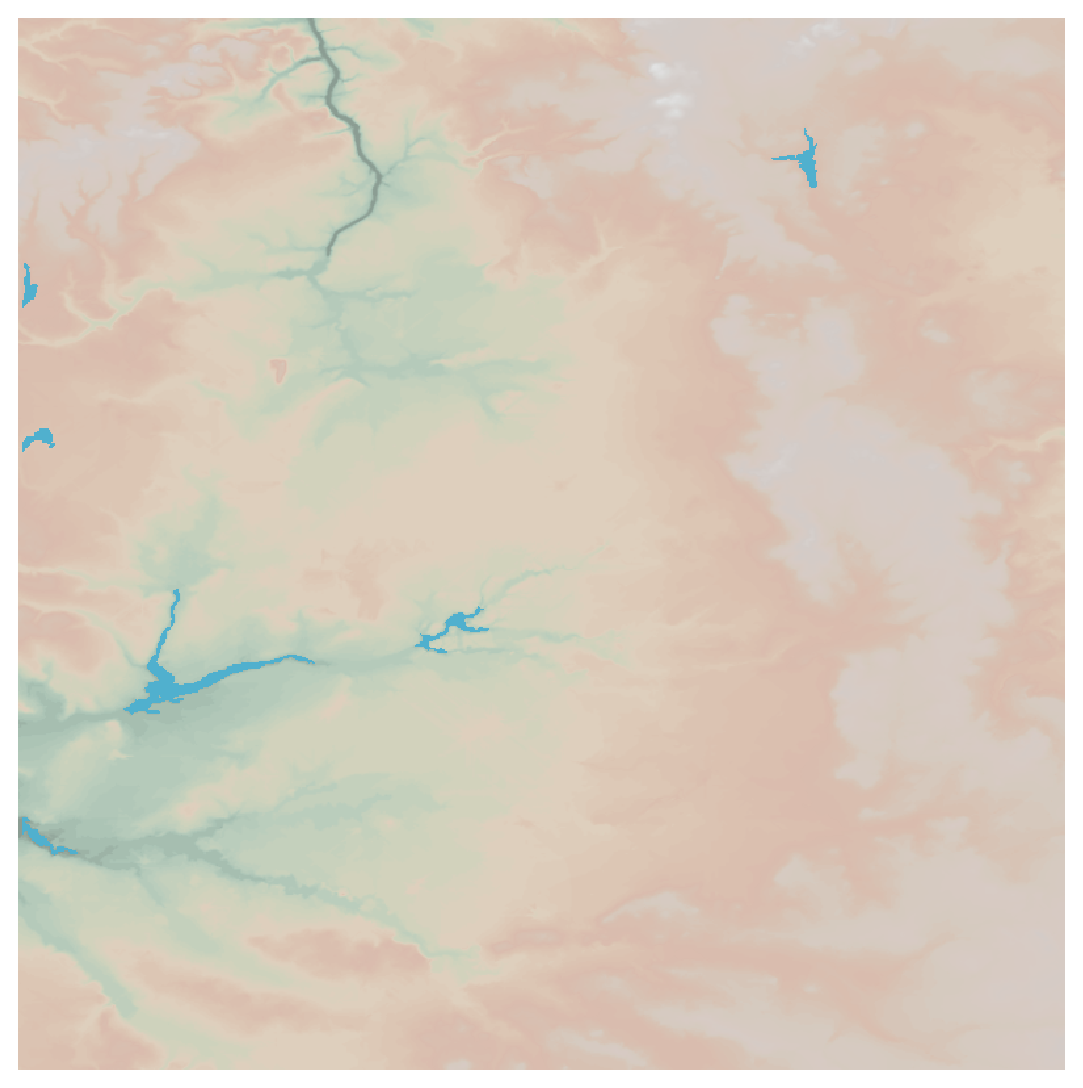
\includegraphics[scale=0.4]{images/network_vis/terrain_lakes.eps}
	\label{fig:terrain_lakes}
}
  \caption{Figure \subref{fig:terrain_no_lakes} shows a sample of terrain visualized without having it lakes detected. Figure \subref{fig:terrain_lakes} then shows the same terrain with its lakes identified and visualized.}
\label{fig:terrain_lake_example}
\end{figure}

\subsubsection{TerrainResolutionChanger Class}
Different digital terrain file formats deal with data of different resolutions.  Some formats are very fine grained while others are rather course.  As an example, DTED files come in varying resolutions, the lowest resolution spaces elevations points every one kilometer while the highest resolution spaces points every thirty meters.  In a simulation the users defined terrain region could be in an arena that spans only a few kilometers.  If using very course terrain data, the number of actual data points the user would receive is very few.  To help the user rectify this problem we have created a tool that allows the users to redefine the resolution of their terrain data very easily.

The user simply needs to load their desired data into our terrain class and use the \textit{TerrainResolutionChanger} to adjust the resolution of the terrain data.  The user only needs to tell the tool what they want the new spacing between adjacent elevation points to be.  The \textit{TerrainResolutionChanger} then interpolates new data points to meet this new resolution requirement.  Interpolating the values between data points offers the user much more valuable data that can be used in running a simulation.  An example of this is illustrated in figure \ref{fig:dted_interpolation}.

\begin{figure}[ht]
\centering
  
\includegraphics[width = 0.5\linewidth]{images/network_vis/dted_interpolation.eps}
  \caption{DTED point interpolation: circles are actual data points, diamonds are interpolated points.  After interpolation the user has much more data to work with.}
\label{fig:dted_interpolation}
\end{figure}

The ability to interpolate new data points allows the user to make queries on the data without having to worry about a limited resolution returning insufficient data for them to calculate meaningful results.

\subsubsection{TerrainReader Class}
The \textit{TerrainReader} class is what handles reading the data from specific digital terrain file formats.  The \textit{TerrainReader} makes use of a specification file in order to define what data to load and how it should be loaded.  Below is a list of the definable parameters for this specification file.

\begin{itemize}
\item \textit{path: } Should contain a full path to the desired terrain data files.  Any standard format for specifying file paths can be used.
\item \textit{bottom\_left: } Specifies the lower left corner of the desired viewport into the given terrain set.  This is specified in latitude and longitude coordinates in the format \textbf{W76.6 N39.9}.
\item  \textit{top\_right: } Specifies the upper right corner of the desired viewport into the given terrain set.  This is specified in latitude and longitude coordinates in the format \textbf{W76.6 N39.9}.
\end{itemize}

All files that contribute to the desired viewport will be loaded in their entirety.  Each file is first loaded into a \textit{TerrainPatch} object, which are simple temporary containers for the file data.  As each file is loaded its \textit{TerrainPatch} is added to a \textit{Terrain} object.  Once all files have been loaded, the \textit{Terrain} object performs a sorting of all the \textit{TerrainPatch} objects based on their latitude and longitude.  Figure \ref{fig:dted_layout} illustrates the proper sorted order of an example set.  Once sorted, the \textit{TerrainPatch} objects are collapsed together into a single matrix within the \textit{Terrain} object, this removes all boundaries that once existed between adjacent files.  If a bounding box was defined in the specification file then this matrix is then trimmed down such that only data that belongs to that desired bounding box remains in memory.

\begin{figure}[ht]
\centering
  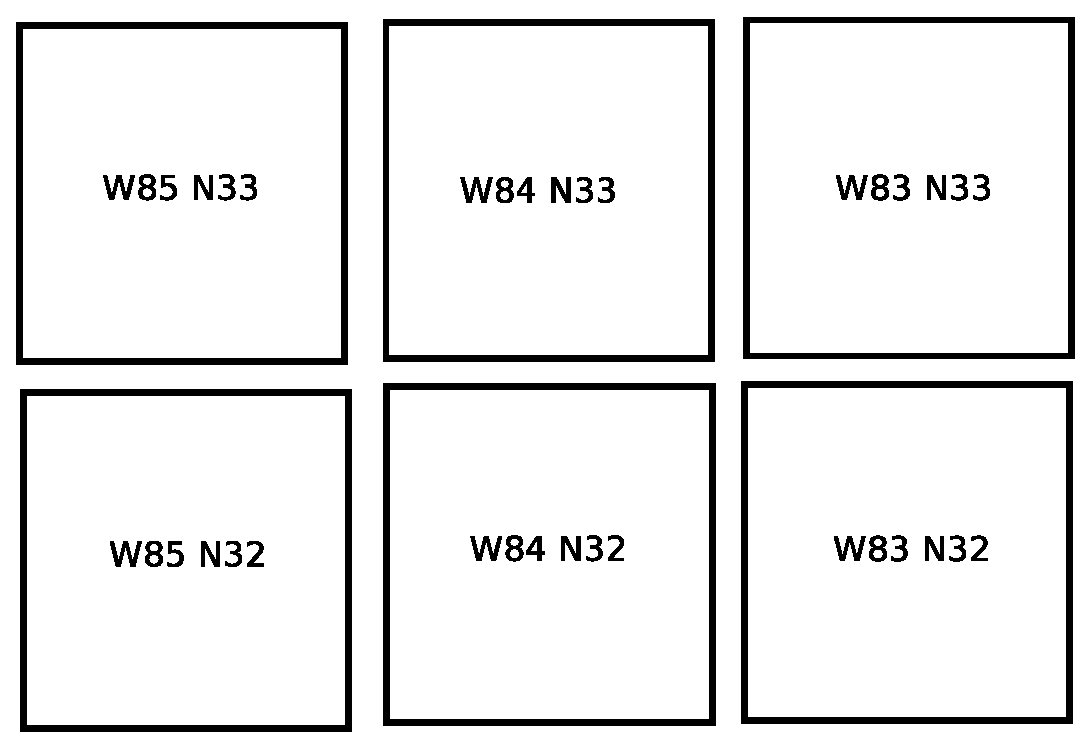
\includegraphics[width=0.5\linewidth]{images/network_vis/dted_file_layout.eps}
  \caption{DTED file ordering}
\label{fig:dted_layout}
\end{figure}


\subsection{Integration with OMAN}
The design of the terrain library allowed for easy integration with OMAN.  OMAN is able to use the terrain library to read in specific terrain to match the desired simulation arena.  The terrain can then be visualized along with the simulated network setup in either 2D or 3D.  In both 2D and 3D visualizations the terrain data is turned into a height map that can be colored in a series of different color schemes.  Figure \ref{fig:terrain_color_schemes} shows a sample of the different color schemes available to visualize the terrain.  

\begin{figure}[ht]
\centering

\subfigure[]{
	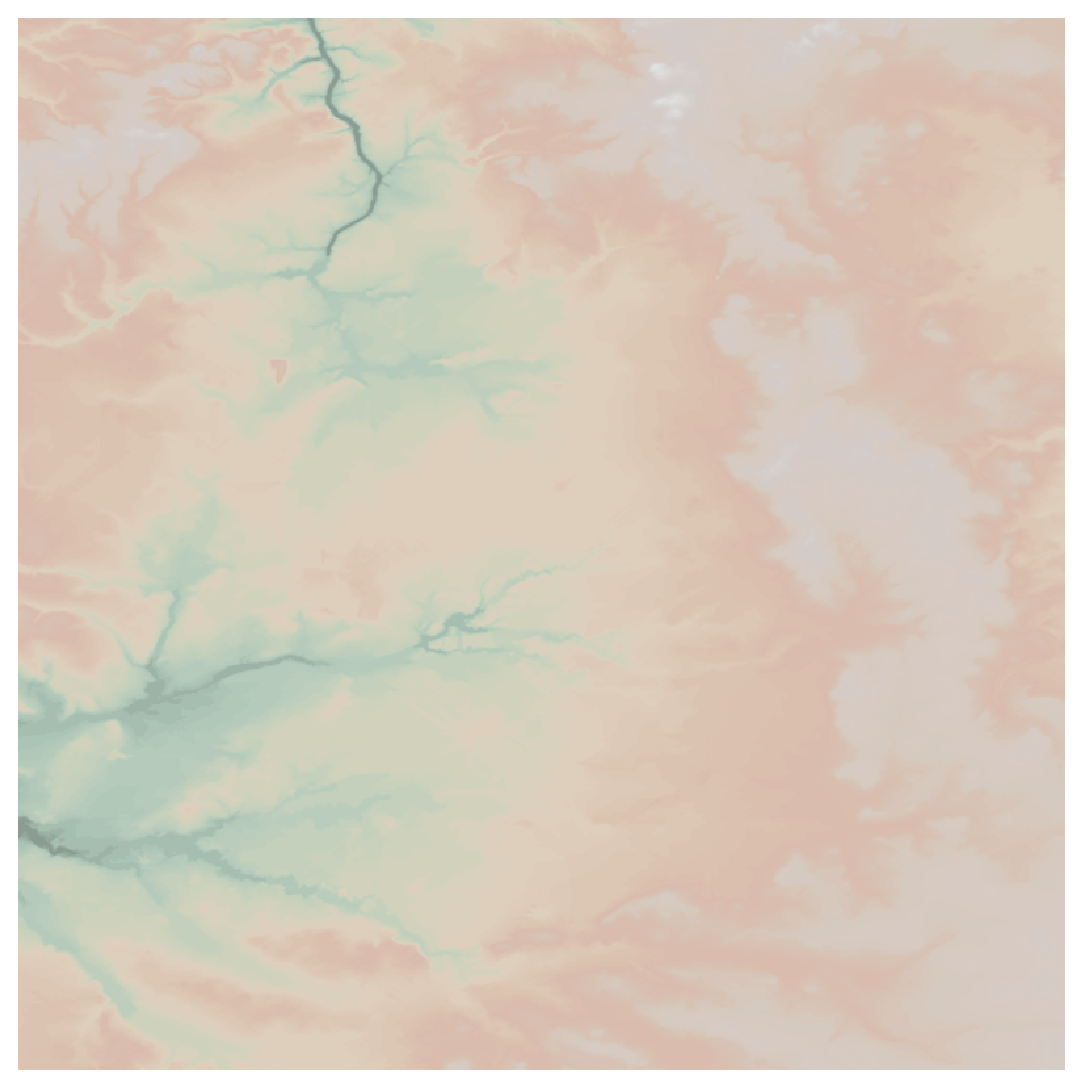
\includegraphics[scale=0.3]{images/network_vis/terrain_no_lakes.eps}
	\label{fig:oman_color_1}
}
\subfigure[]{
	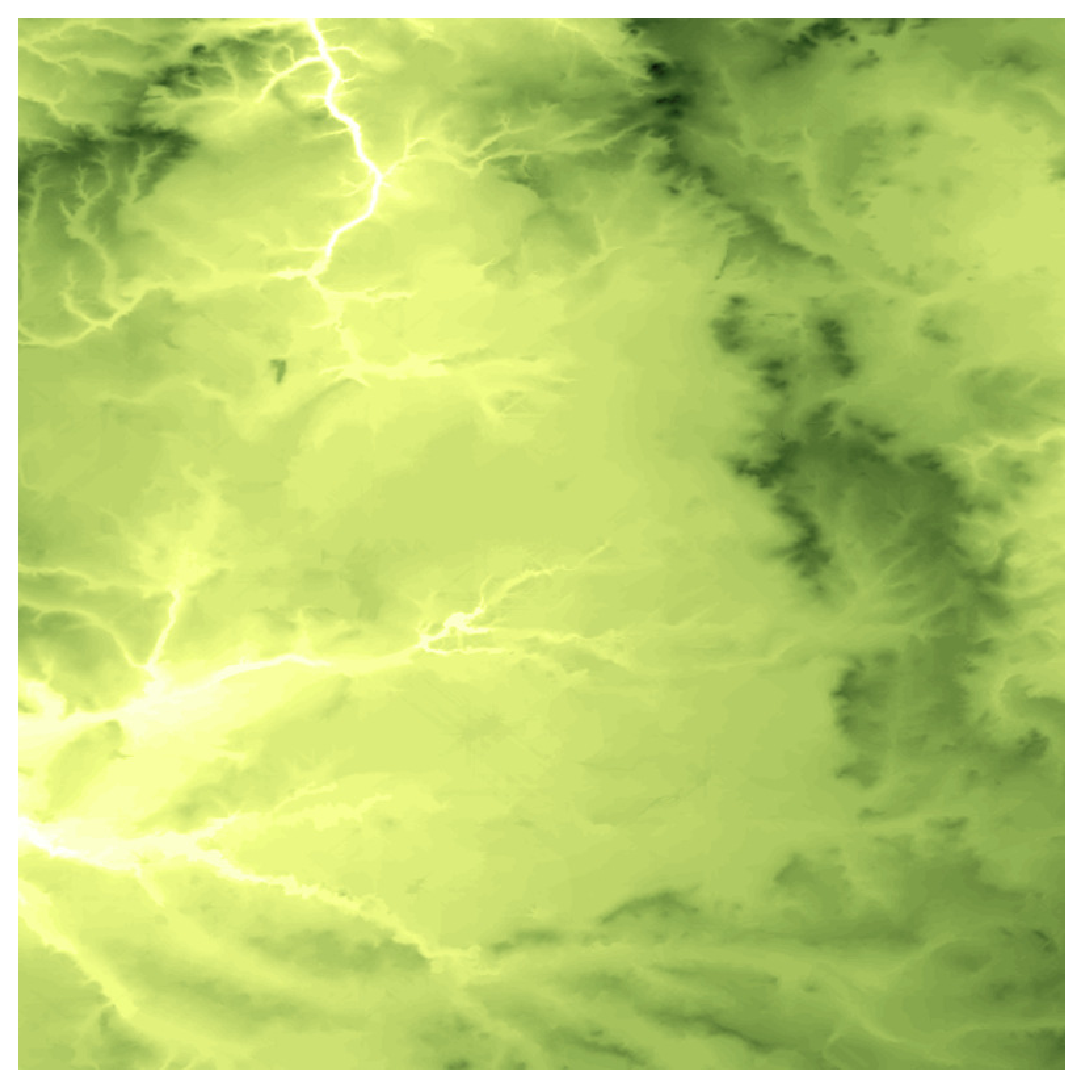
\includegraphics[scale=0.3]{images/network_vis/terrain_color_scheme_2.eps}
	\label{fig:oman_color_2}
}
\subfigure[]{
	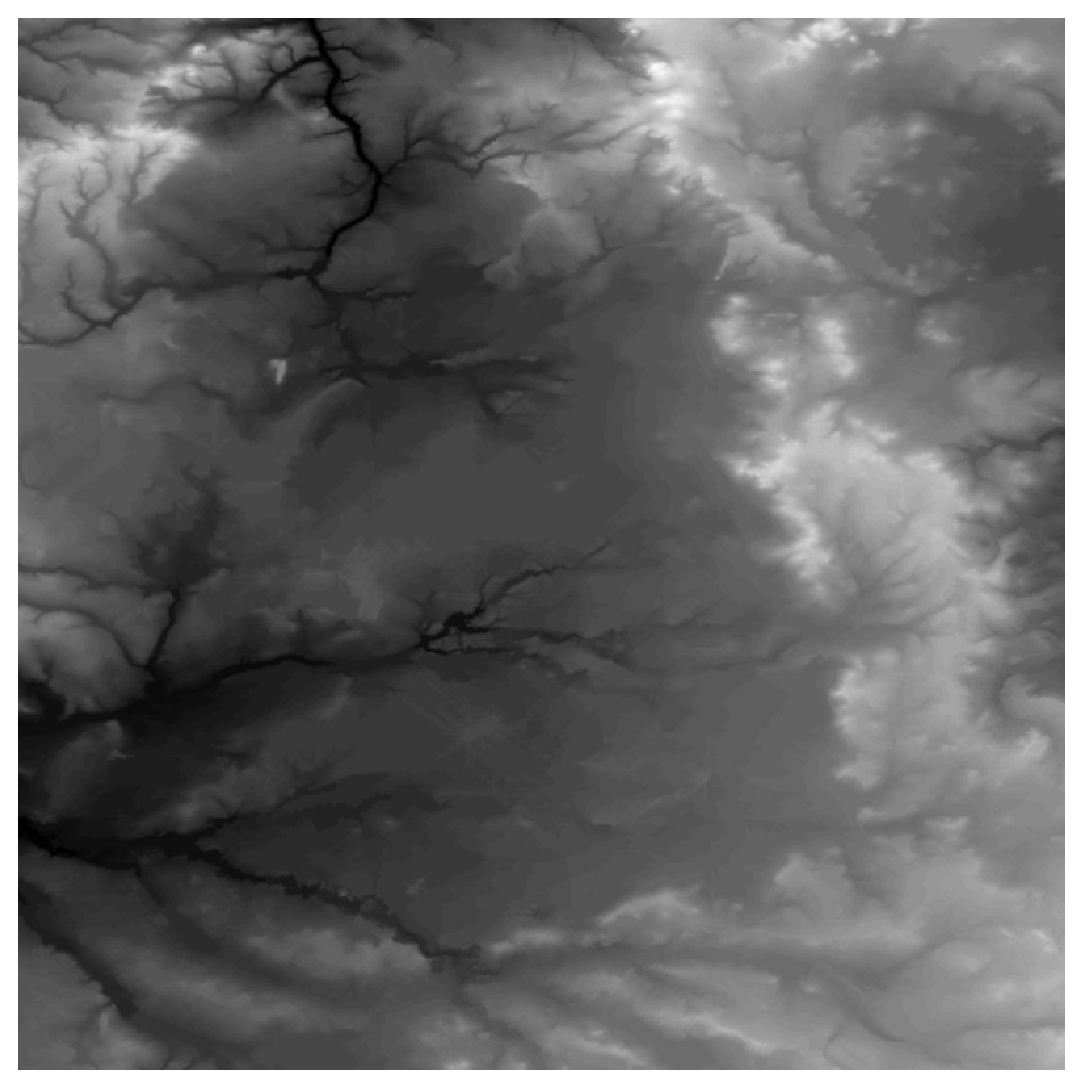
\includegraphics[scale=0.3]{images/network_vis/terrain_color_scheme_3.eps}
	\label{fig:oman_color_3}
}
\subfigure[]{
	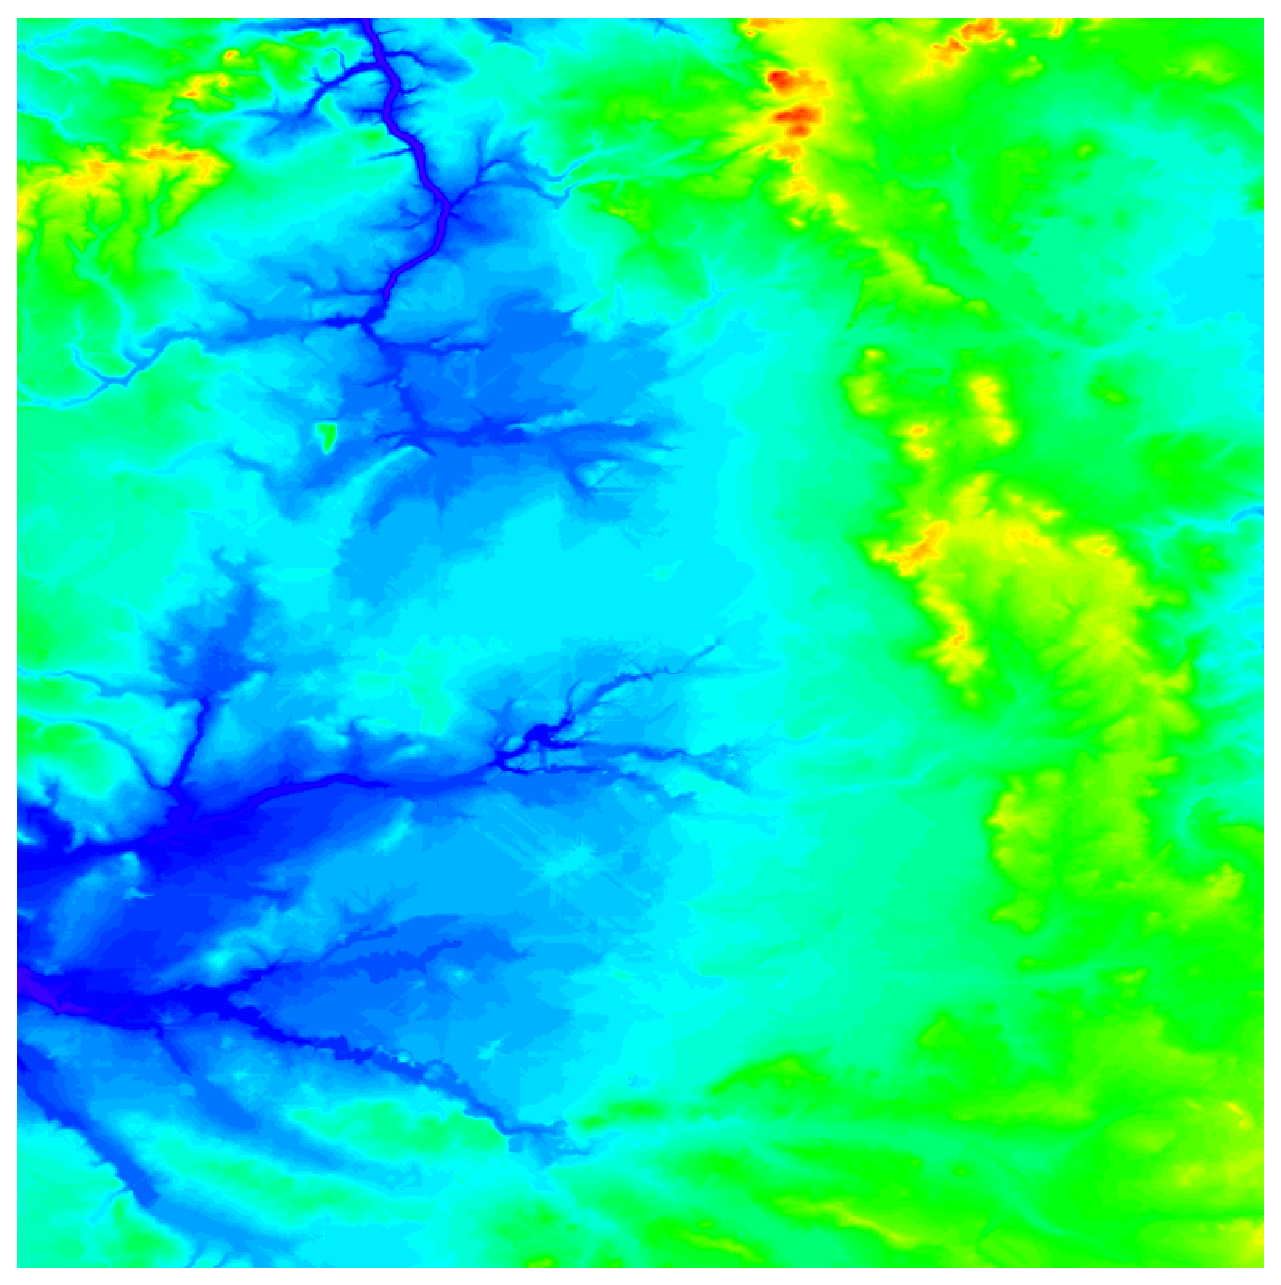
\includegraphics[scale=0.3]{images/network_vis/terrain_color_scheme_4.eps}
	\label{fig:oman_color_4}
}
  \caption{These figures illustrate 3 of the different possible color maps that can be applied to the visualization of the terrain in 2D. \subref{fig:oman_color_1} is a standard terrain color gradient, \subref{fig:oman_color_2} is a forest gradient shifting from white to green, \subref{fig:oman_color_3} is a standard gray scale gradient, and \subref{fig:oman_color_4} is an HSV color gradient starting at blue and sweeping to red.}
\label{fig:terrain_color_schemes}
\end{figure}

Users can also choose what minimum and maximum elevation values to use when computing the color schemes.  They can choose to use the current terrains minimum and maximum values, the known highest and lowest terrain values in the United States, or the known highest and lowest terrain values in the world.  Once the terrain has been converted into a color coded height map it is ready for display.  

\paragraph{2D Visualization}
In 2D this height map is simply turned into an image and used as a background on which the network layouts can be placed on top of.  Figures \ref{fig:oman_flow_graph_2D} shows an OMAN flow graph overlayed on top of a terrain region while Figure \ref{fig:oman_physical_graph_2D} shows an OMAN physical graph.  Visualizing the graph structures on top of a map of the terrain can give the users more insight into how and why the simulation produced its results.  An example of this would be in a simulated movement graph, where nodes simulate intelligently moving around a given arena, the addition of visual terrain data can show whether the node movements are logical when coping with terrain obstacles.

\begin{figure}[ht]
\centering

\subfigure[OMAN flow graph]{
	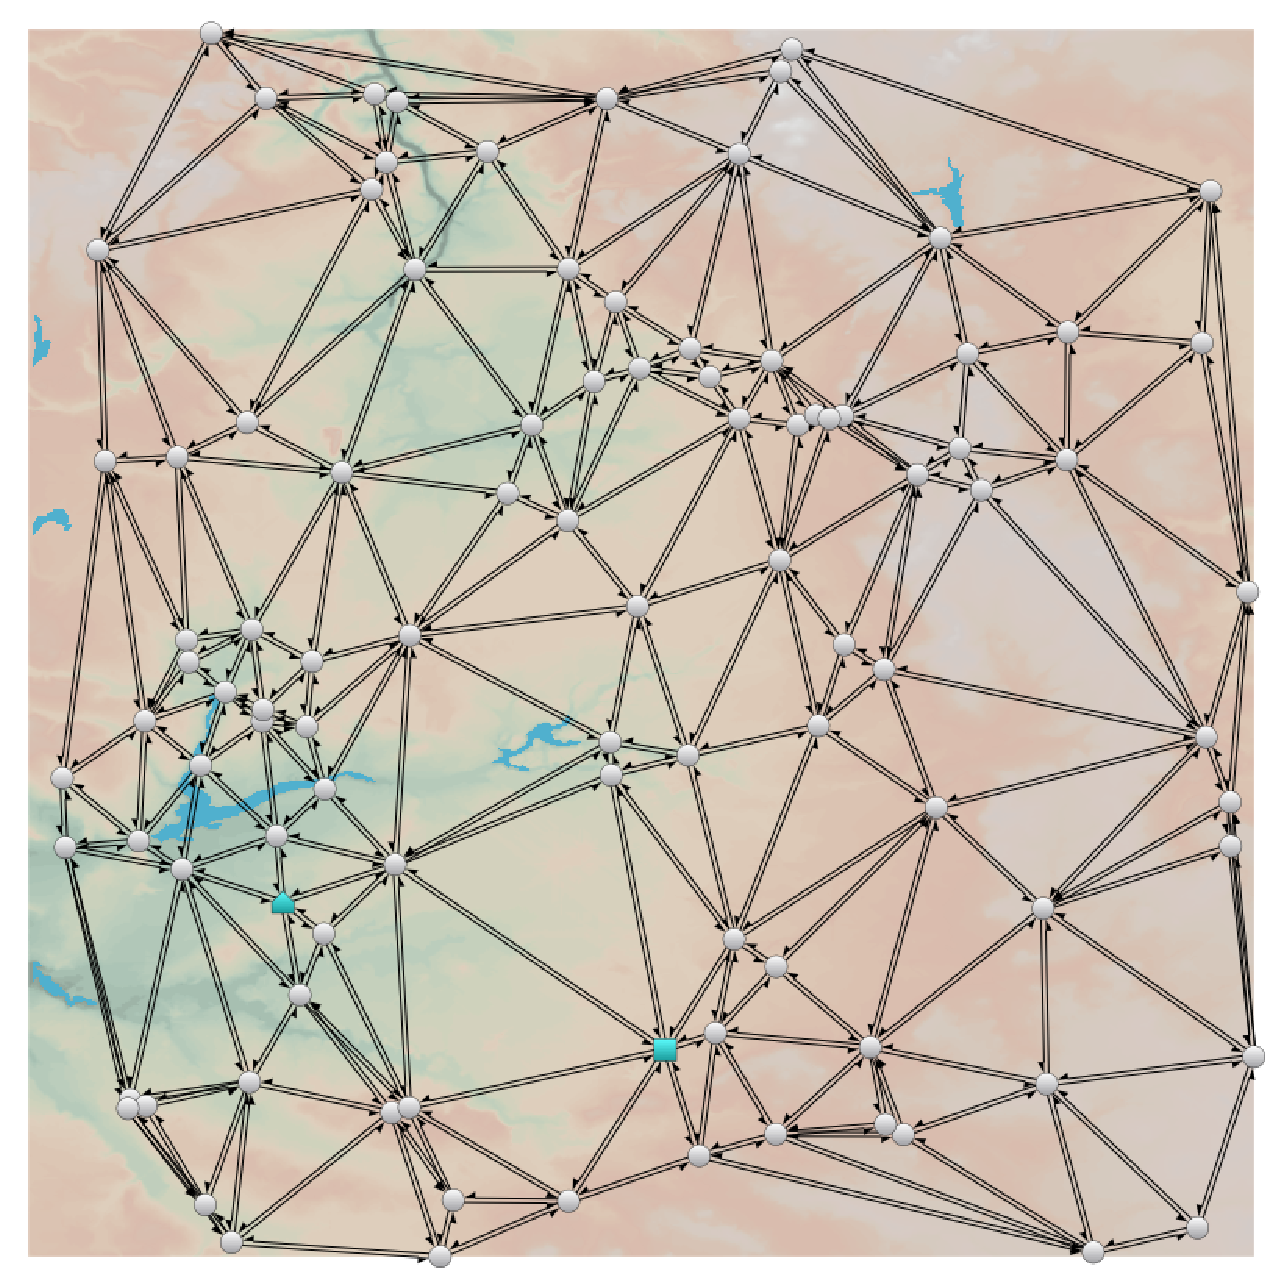
\includegraphics[scale=0.33]{images/network_vis/terrain-with-flow-graph_1.eps}
	\label{fig:oman_flow_graph_2D}
}
\subfigure[OMAN physical graph]{
	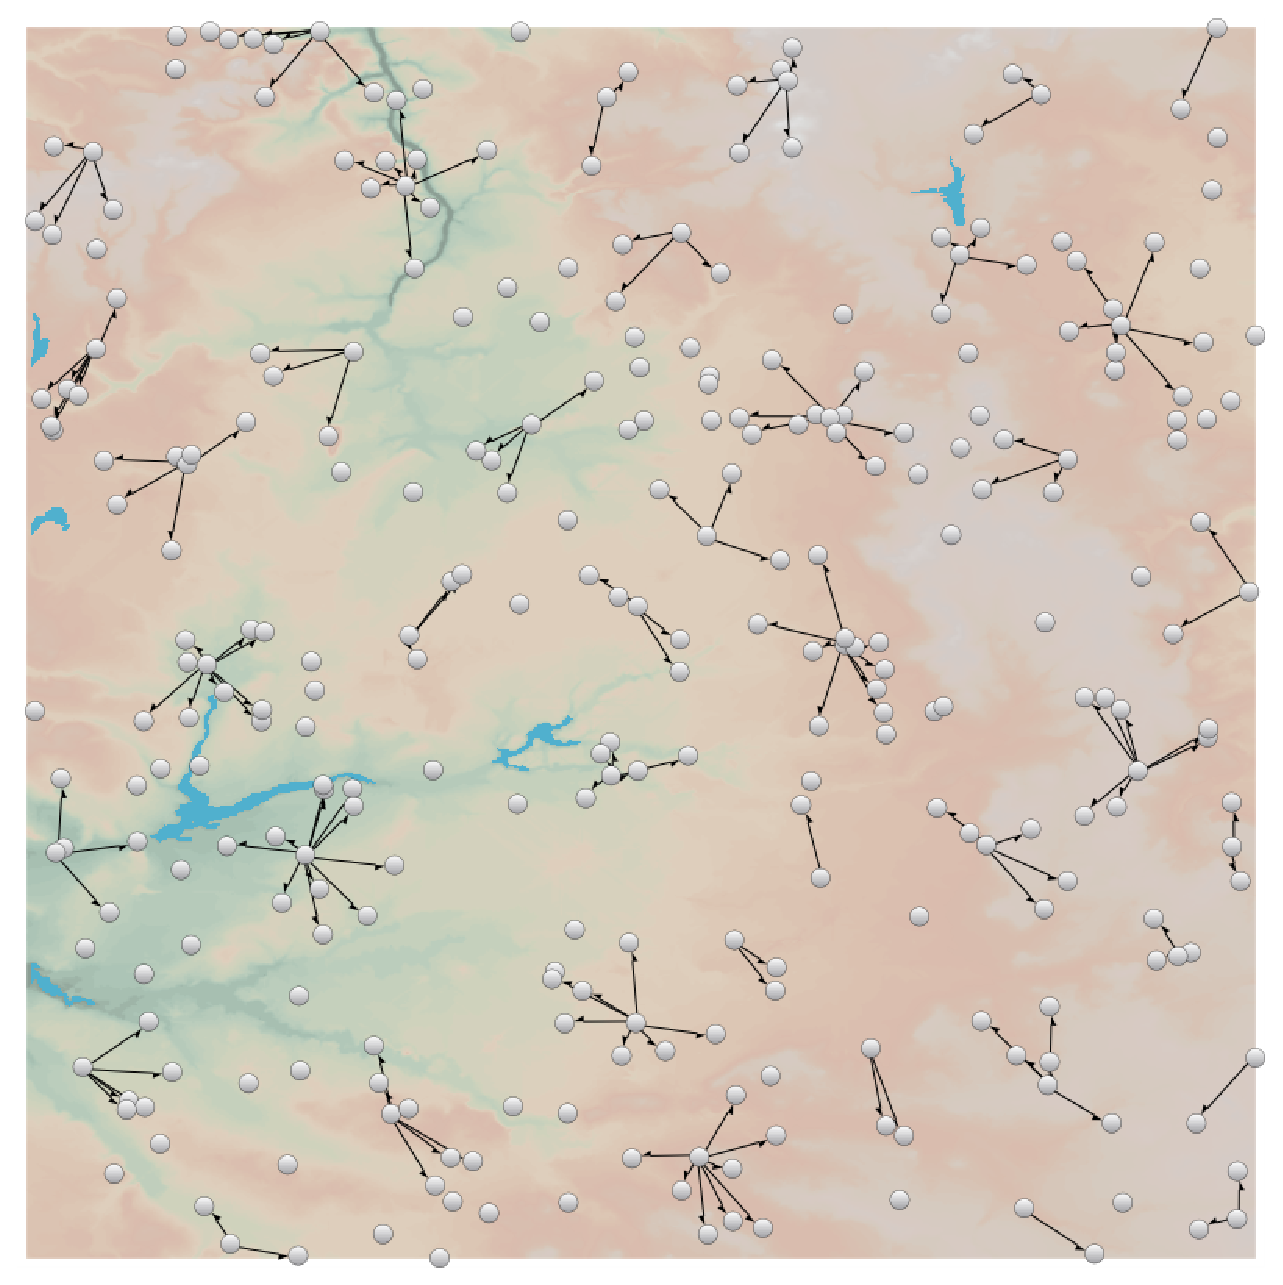
\includegraphics[scale=0.33]{images/network_vis/terrain-with-physical-graph.eps}
	\label{fig:oman_physical_graph_2D}
}
  \caption{Figures showing OMAN network graphs visualized on top of terrain}
\label{fig:oman_graphs_on_terrain}
\end{figure}

\paragraph{3D Visualization}
Although 2D visualizations do provide useful information, looking at a height map is not always intuitive and does not always present all of the information.  The visualization of terrain really benefits from 3D visualization.  Just the added dimension does not provide all the potential benefits, the inclusion of interactivity in the 3D world provides the richest visualization for this data.  Figure \ref{fig:3d_terrain_overhead} shows a simple overhead view of a physical graph visualized on a given terrain arena in 3D.  Looking at this figure we don't get the sense we have gained much in going from 2D to 3D.  We still see a graph visualized on top of a terrain arena but now with the contours of the terrain and positioning of the nodes better visualized.

\begin{figure}[ht]
\centering
  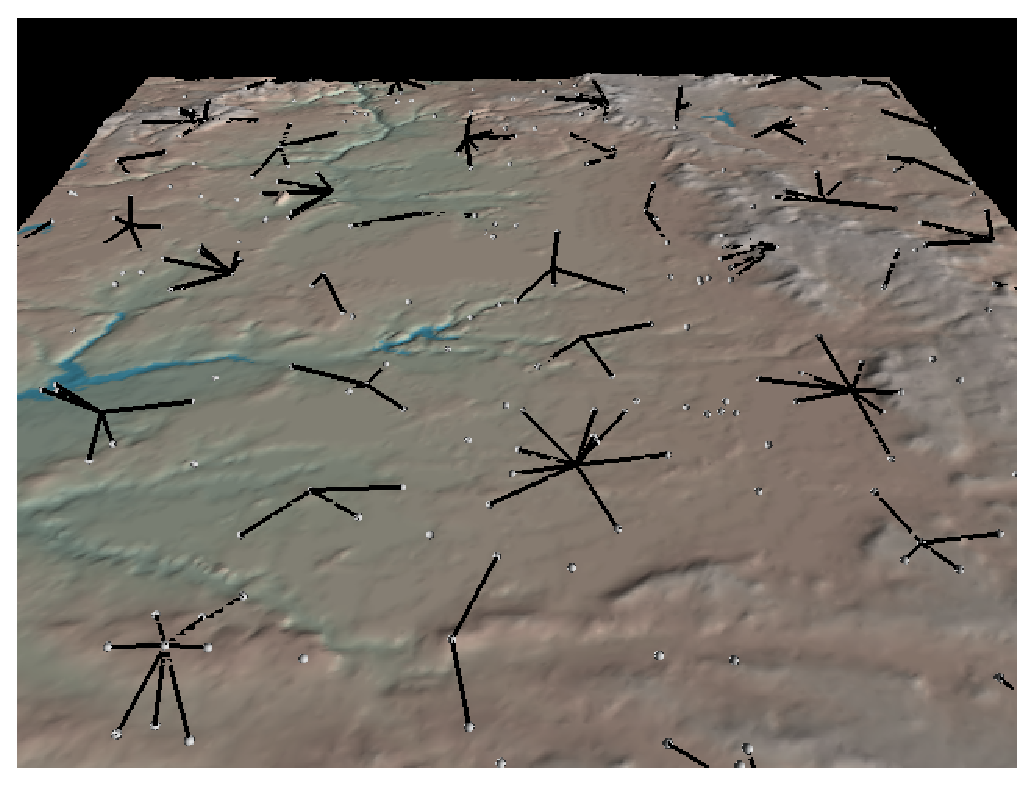
\includegraphics[scale=0.75]{images/network_vis/3D_terrain.eps}
  \caption{Terrain visualization in 3D, overhead view}
\label{fig:3d_terrain_overhead}
\end{figure}

The use of the available interactivity really shows the usefulness of this type of visualization.  In this visualization the user has complete control and freedom of movement with the camera.  The Figures \ref{fig:3d_terrain_closeup_1} and \ref{fig:3d_terrain_closeup_2} show two different perspectives of portions of the terrain from Figure \ref{fig:3d_terrain_overhead}.  These views are much easier to understand and comprehend than a 2d height map visualized under the plot of a graph.  The features of the terrain are easily distinguishable and the effects they have can be easily seen when we zoom into the environment.

\begin{figure}[ht]
\centering
\subfigure[]{
	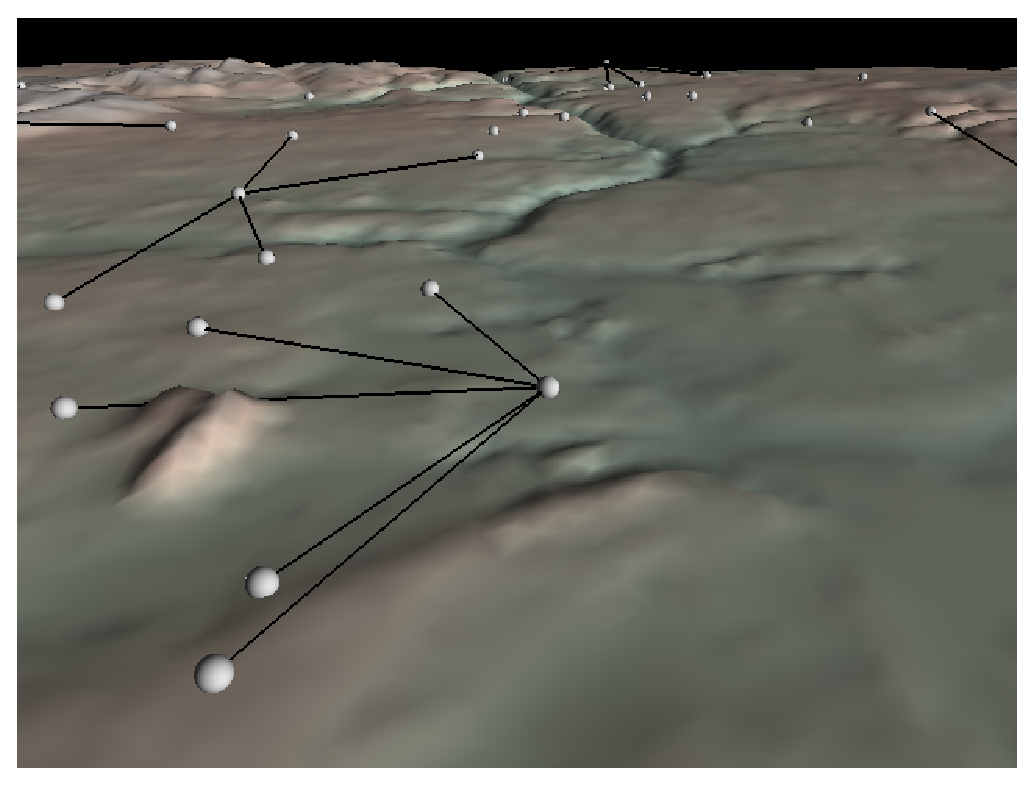
\includegraphics[scale=0.40]{images/network_vis/3d_terrain_closeup_1.eps}
	\label{fig:3d_terrain_closeup_1}
}
\subfigure[]{
	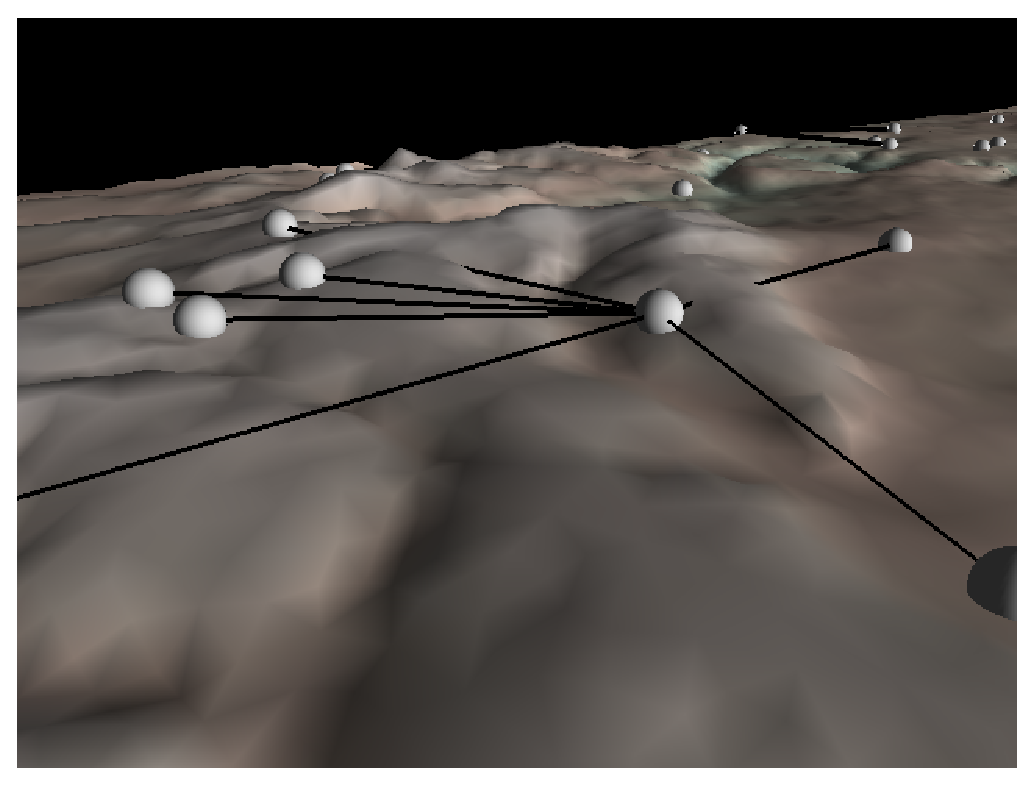
\includegraphics[scale=0.40]{images/network_vis/3d_terrain_closeup_2.eps}
	\label{fig:3d_terrain_closeup_2}
}
\subfigure[]{
	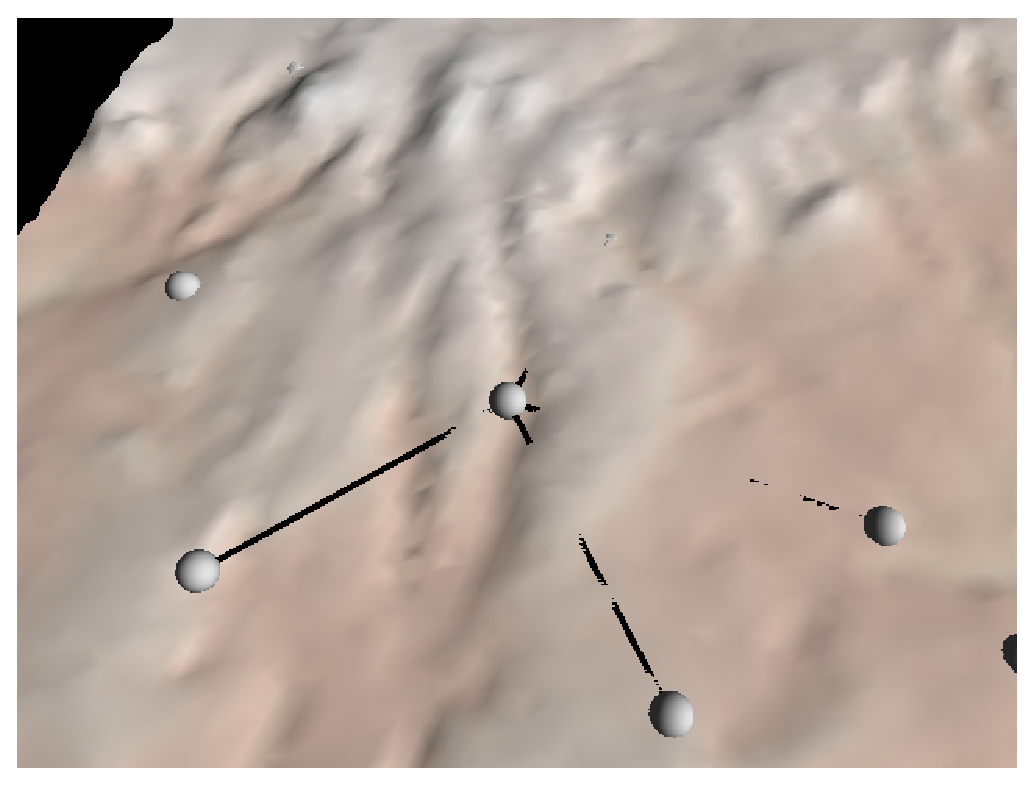
\includegraphics[scale=0.40]{images/network_vis/terrain_obstructions_2.eps}
	\label{fig:3d_terrain_obstruction_2}
}
\subfigure[]{
	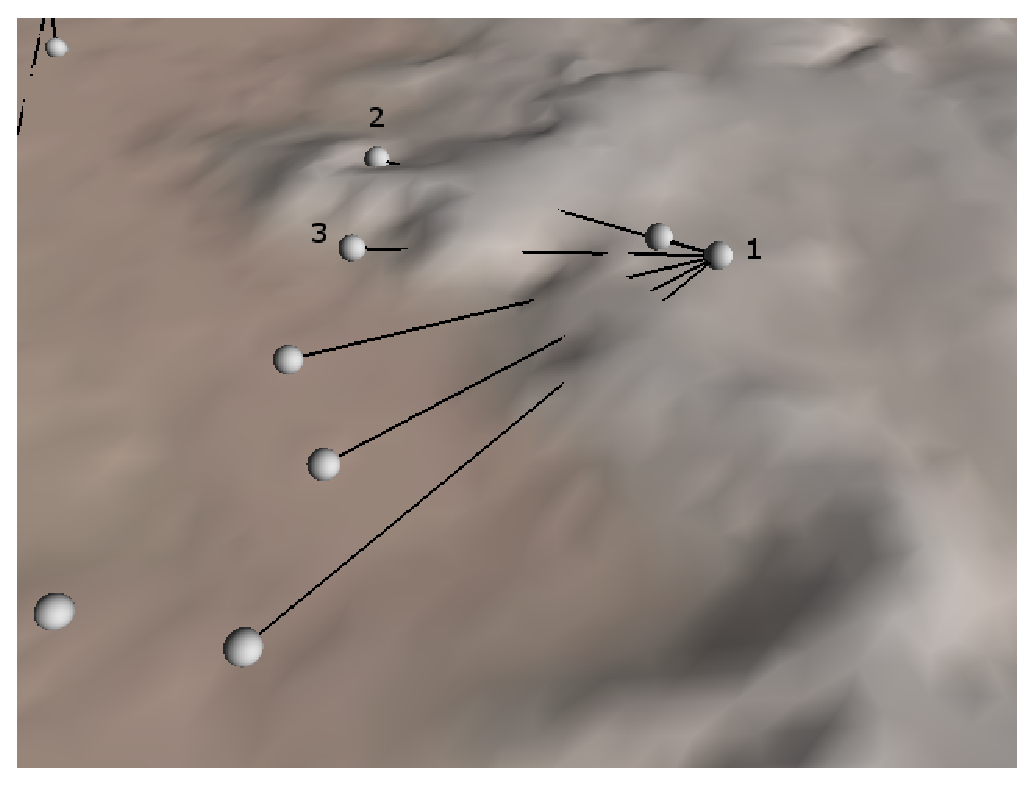
\includegraphics[scale=0.40]{images/network_vis/terrain_obstructions_3.eps}
	\label{fig:3d_terrain_obstruction_3}
}
  \caption{Figures showing a zoomed in view of portions of 3D terrain with portions of a physical graph visualized on top of them.}
\label{fig:3d_terrain_closeups}
\end{figure}

An example of these effects is more clearly illustrated in Figures \ref{fig:3d_terrain_obstruction_2} and \ref{fig:3d_terrain_obstruction_3}.  In Figure \ref{fig:3d_terrain_obstruction_2} we can see nodes 2 and 3 are hidden behind elements of the terrain which may cause trouble in their connections with node 1.  We see a similar situation in Figure \ref{fig:3d_terrain_obstruction_3}.  These situations are not as easily identifiable when visualized in 2D.  Although one can zoom into a static 2d image, it is more difficult to interpret the exact values on a height map and try and draw conclusions that way.  Seeing these situations in 3D makes it quick and easy to directly see the result.

One of the only troubles we encounter in the 3D view of this data is that when looking at the terrain at a whole it is easy for the nodes and edges to get lost in the details of the terrain.  To alleviate this problem, nodes and edges can be scaled up in size so that they are easily visible when the view is zoomed out.  This feature is illustrated in Figures \ref{fig:3d_terrain_node_scale}.

\begin{figure}[ht]
\centering
\subfigure[]{
	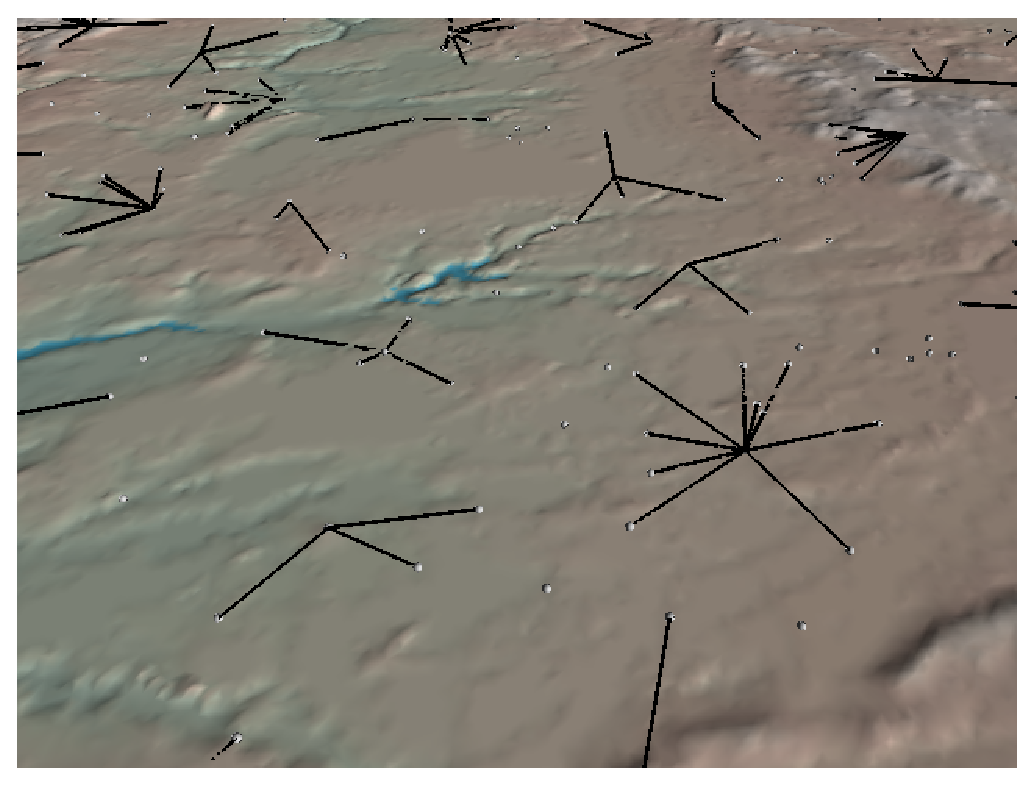
\includegraphics[scale=0.40]{images/network_vis/3d_terrain_node_scale_1.eps}
	\label{fig:3d_terrain_node_scale_1}
}
\subfigure[]{
	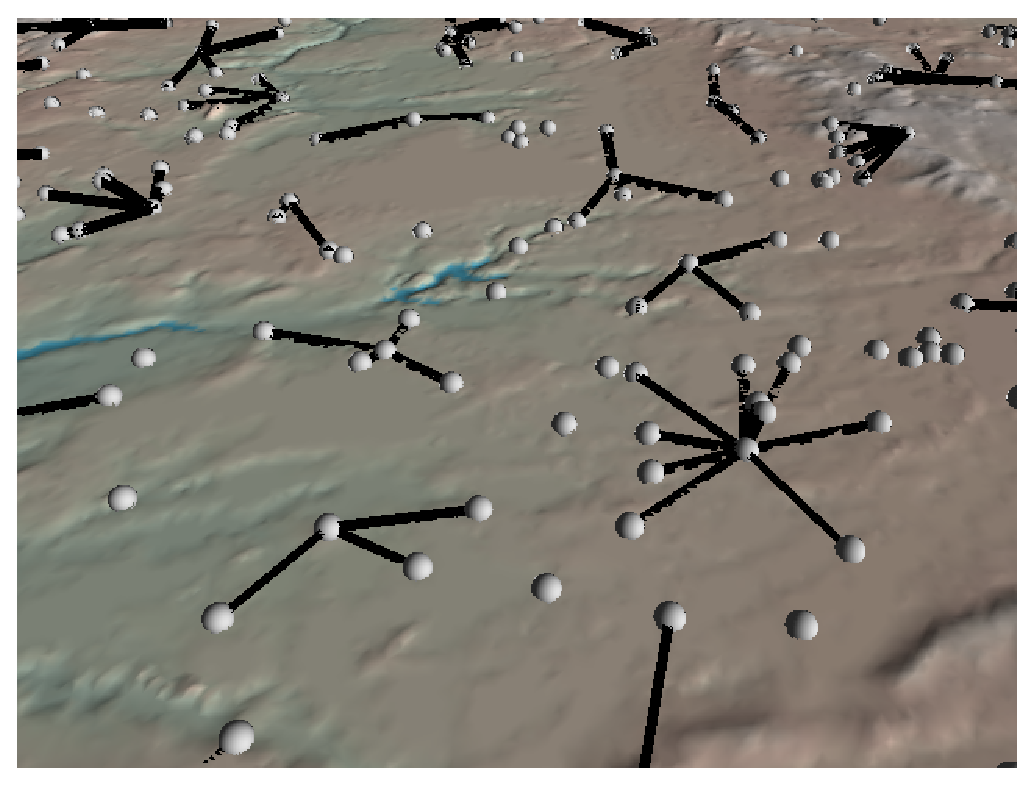
\includegraphics[scale=0.40]{images/network_vis/3d_terrain_node_scale_2.eps}
	\label{fig:3d_terrain_node_scale_2}
}
  \caption{\subref{fig:3d_terrain_node_scale_1} shows the nodes and edges at normal size.  \subref{fig:3d_terrain_node_scale_2} shows the nodes and edges scaled up for better visibility.}
\label{fig:3d_terrain_node_scale}
\end{figure}

\section{Conclusion}
In this chapter we have discussed two network visualizations that have been implemented in the OMAN adhoc wireless network simulator.  First, we have shown a method for providing a visual representation of the signal radiation patterns of transmitting nodes.  Along with this we have provided a visual representation of the regions of acceptably high SINR which allow a feasible channel to exist.  Each of these visualizations are done for both certain and uncertain environments.

Our second visualization presented is the use of digital terrain data to improve the visualization of network simulation results.  We started by discussing the terrain library that was implemented in support of adding digital terrain data into OMAN.  With that we then discussed the different 2D and 3D visualization options this then added to OMAN.

\section{Future Work}
In future work we hope to develop further methods of meaningfully visualizing other layers of the network model.  The integration of different visualizations together would also be a worth while exploration.  The display of the signal radiation patterns overlayed onto the 3D display of the network with its terrain could help to reveal further information about the simulation results.  We would also like to further develop the interactivity of the 3D displays.

